\chapter{Methodology}\label{chapter:methodology}


% need change
This chapter discusses mathematical principles of models used in the thesis. The kernel metrics, basic dataset input for training, data processing methods and three prediction models are covered respectively, along with the intuition behind the methodology. In Section~\ref{sec:data-flow}, I summarize the whole data flow and how the three parts are connected. 

\section{Aggressive Trade: Target Variables}
In the FX trading market, once two orders get matched, the information is clearly recorded in trade book data, including the filling price, volume and direction where the order triggers. There are two ways of trading. Traders may aggressively participate and take out orders which are waiting in the order book. This happens when traders are eager to get trades done, putting more priority in time than price. Normally the filling price for this aggressive trade is higher (lower) than the mid-price and across the spread to touch even more aggressive price. In contrast to aggressive trade, it is also common that a trader just put forward a limit order and let it queue in the order flow. After positive market movements, the best bid/ask price matches the order price, the order is likely to get filled if it has the top priority. If the orders are matched, this information is also recorded in the trade book, but with a filling price at the best bid/ask. If it fails to match, it continues to stay in the order book and deepen the order book flow. Besides these two active trading situations, there are plenty of orders silently being submitted or staying and can not find any corresponding records in the trade book at the same timestamp. 

Two targets are provided in Section~\ref{sec: alpha} and Section~\ref{sec: aflag} which describe the trader behaviors in different situations. In the first section I introduce a continuous method to better understand the changing logic, while in the second section the real modeled target is shown and explained.

\subsection{Aggressiveness} \label{sec: alpha}
How aggressive a trader wants to submit orders and match existing orders is worth to discuss in this research. The purpose of defining it is to provide insight into aggressive trade behavior. It is not used in the model itself. In order to quantify and measure the level, I introduce a metric called \textit{aggressiveness}, denoted by $\alpha$:

\begin{equation}
    \alpha = \frac{P_F - P_B}{P_B}
    \label{eq: aggressiveness}
\end{equation}

$\alpha$ measures the aggressiveness of each trade. $P_F$ is the filling price at the time of the trade, and $P_B$ is the reference price used to determine whether a trade is aggressive. In this context, I set the benchmark as the previous mid-price in the order book, i.e., the mid-price from the most recent update before the current trade. For example, if a trader wants to buy and places an order above the mid-price to grab existing ask orders, this behavior is considered aggressive. The comparison is made against the last observed mid-price before the trader submitted the order. 

As shown in Equation~\ref{eq: aggressiveness}, for instance, on the bid side, $\alpha$ is positive if the filling price is higher than the benchmark price. This indicates that a trader is willing to buy at a price above the benchmark. Conversely, $\alpha$ is negative if the trader buys at a price below the benchmark. Similarly, on the ask side, $\alpha$ is negative when a trader sells at a price lower than the benchmark, and positive when the selling price exceeds the benchmark. Therefore, an aggressive trade is defined when $\alpha$ is positive on the bid side and negative on the ask side. When there are no trade records, $\alpha$ is assigned a value of 0. The meanings of different $\alpha$ values are summarized in Table~\ref{tb: alpha_meaning}. It is important to note that $\alpha$ is introduced only to help understand the aggressive trade situation and is not used in the modeling process. 

\begin{table}[h] 
    \centering 
    \begin{tabular}{lll} 
        \toprule 
        \textbf{$\alpha$} & \textbf{Meaning} & \textbf{Data Type} \\ 
        \midrule 
        $ > 0$ & Aggressive bid side trades, or passive ask side trades & Float \\
        $ < 0$ & Aggressive ask side trades, or passive bid side trades & Float \\ 
        $ = 0$ & No trades & Float \\  
        \bottomrule 
    \end{tabular} 
    \caption{Interpretation of $\alpha$ in Different Contexts}
    \label{tb: alpha_meaning}
\end{table}

\subsection{Binary Label for Aggressive Trade} \label{sec: aflag}
However, it is important to note that in the backtesting context at MN, I pay little attention to how aggressive a trader is, whether and when an aggressive trade will occur is more critical. Therefore, based on the $\alpha$, a binary target, called aggressiveness flag, denoted as $\bar{\alpha}$, is introduced. The direction of the trade is not considered by $\bar{\alpha}$ because I assume that traders will adjust order direction according to our order submission dynamically. $\bar{\alpha}$ is set to $0$ if no trade takes place or $\alpha$ is positive in ask side and negative in bid side takes at a given timestamp in the order book, and $1$ if $\alpha$ is possible in bid side and negative in ask side. 
\begin{table}[h] 
    \centering 
    \begin{tabular}{lll} 
        \toprule 
        \textbf{$\bar{\alpha}$} & \textbf{Meaning} & \textbf{Data Type} \\ 
        \midrule 
        $ = 1$ & Aggressive trades & Integer \\
        $ = 0$ & Both passive trades and cases where no trade occurred & Integer \\  
        \bottomrule 
    \end{tabular} 
    \caption{Interpretation of $\bar{\alpha}$ in Different Contexts}
    \label{tb: aflag_meaning}
\end{table}
In Table~\ref{tb: aflag_meaning}, I get binary flag $\bar{\alpha}$ which contains $1$ and $0$. It is reduced to a classification problem to solve by models, but the complexity of this issue comes from the class imbalance and feature dependencies. I will discuss them in the following contents in detail.



\section{Data Processing Methods}
% This part describes the dataset used for machine learning training, and resampling and rescale methods
The original order book data and trade book data (Table~\ref{tb: order book data description} and Table~\ref{tb: trade book data description}) fetched from Snowflake and exchange database are too raw to be modeled. In this section, I proceed to discuss methods that are used in data processing. First I discuss feature engineering. It is the process of transforming raw data into meaningful features that enhance the performance of machine learning models. I get effective features based on the calculation of spread, midprice and volume. Then another standard problem: class imbalance is analyzed.

Specifically, in Section~\ref{sec: training data}, I provide basic dataset for model training, test, estimation and prediction, along with specific formulas for certain features. The theoretical solution for extreme class imbalance is established in Section~\ref{sec: class imbalance}.

\subsection{Feature Engineering: Basic Dataset for Model Training} \label{sec: training data}
In selecting which features to generate, I inherit indicators from original order book and trade book, then extend them to get further features. The target discussed in Section~\ref{sec: aflag} is included as the basic dataset.

\begin{table}[h] 
    \centering 
    \begin{tabular}{lll} 
        \toprule 
        \textbf{Column} & \textbf{Description} & \textbf{Data Type} \\ 
        \midrule 
        $\bar{\alpha}$ & Binary flag & Integer \\
        $T$ & Timestamp of the snapshot in HH:MM.SSS & String \\
        \text{DIRECTION} & Bid($1$) or ask($-1$) trades & Integer \\
        $S$ & Difference between best ask and bid & Float \\
        $M$ & Middle price of best ask and bid & Float\\
        $V_A ^ {1}$ & Volume at best ask & Integer\\
        $V_B ^ {1}$ & Volume at best bid & Integer \\
        %$\alpha$ & How aggressive a trade is & Float \\ 
        %$\tau$ &  &  \\
        $\bar{\delta}_S$ & Average absolute spread change over the past 50 ticks & Float \\
        $\bar{\delta}_M$ & Average absolute mid-price change over the past 50 ticks & Float \\
        $\sigma_S$ & Volatility of spread over the last 50 ticks & Float \\
        $\sigma_M$ & Volatility of mid-price over the last 50 ticks & Float \\
        $r_V$ & Volume imbalance between best ask and bid & Float \\
        \bottomrule 
    \end{tabular} 
    \caption{Overall Dataset for Modeling}
    \label{tb: overall dataset for training}  
\end{table}
In the Table~\ref{tb: overall dataset for training}, capitalized terms refer to variables obtained directly from the order book and trade book data, including timestamp($T$), spread($S$), mid-price($M$), volume($V_A^{1}$, $V_B^{1}$). $T$ represents the time snapshot calculated relative to millisecond.

The last five features ($\bar{\delta}_S$, $\bar{\delta}_M$, $\sigma_S$, $\sigma_M$, $r_V$) are calculated from spread, mid-price or volume based on common factors which display order flow dynamics. $\bar{\delta}_S$ and $\bar{\delta}_M$ measure the local average absolute change over. They both capture the rapid changes in the cost of executing trades, directly related to liquidity changes in real market LOB dynamics. Specifically, $\bar{\delta}_M$ is useful to simulate realistic microstructure scenarios where aggressive trades tend to cluster, such as around price jumps. A 50-tick window is commonly used in high-frequency time series data because it effectively represents the local market environment without unnecessary noise or excessive smoothing. $\bar{\delta}_S$ and $\bar{\delta}_M$ can be formulated as follows:

\begin{equation}
    \bar{\delta}_{S_t} = \frac{1}{50} \sum_{i=0}^{49} \left| S_{t-i} - S_{t-i-1} \right| 
    \label{eq: spread change} 
\end{equation}
\begin{equation}
    \bar{\delta}_{M_t} = \frac{1}{50} \sum_{i=0}^{49} \left| M_{t-i} - M_{t-i-1} \right|
    \label{eq: midprice change} 
\end{equation}

Mid-price realized volatility affects order flows \citep{OrderAggressiveness2010}, thus $\sigma_M$ is used to depict the variability of mid-price changes. As defined in Equation~\ref{eq: midprice vola} and \ref{eq: spread vola}, standard deviation of mid-price changes and spread changes are calculated over a rolling window of 50 ticks. Spread factor $\sigma_S$ is also included because it reflects the consistency and variability of liquidity conditions.

\begin{equation}
    \sigma_{S_t} = \sqrt{\frac{1}{49}\sum_{i=0}^{48}\left((S_{t - i}-S_{t - i - 1})-\bar{\delta}_{S_t}\right)^2}
    \label{eq: spread vola}
\end{equation}

\begin{equation}
    \sigma_{M_t} = \sqrt{\frac{1}{49}\sum_{i=0}^{48}\left((M_{t - i}-M_{t - i - 1})-\bar{\delta}_{M_t}\right)^2}
    \label{eq: midprice vola}
\end{equation}

Higher $\bar{\delta}$ ($\bar{\delta}_S$ and $\bar{\delta}_M$) indicates that the market experiences frequent, sizable changes, with higher $\bar{\delta}_S$ reflecting unstable liquidity, and higher $\bar{\delta}_M$ showing active price discovery and increased market uncertainty. Conversely, lower $\bar{\delta}$ values signify stability, with lower $\bar{\delta}_S$ indicating consistent liquidity, and lower $\bar{\delta}_M$ suggesting calmer, more stable price movements.

Higher $\sigma$ ($\sigma_M$ and $\sigma_S$) represents greater variability and unpredictability in the market, with higher $\sigma_{S}$ highlighting liquidity risk, and higher $\sigma_{M}$ means significant fluctuations and uncertainty in the mid-price. Lower $\sigma$ denotes more predictable conditions, where lower $\sigma_{S}$ indicates stable liquidity conditions and lower $\sigma_{M}$ reflects reduced price uncertainty and market stability.

$r_V$ represents the relative imbalance between the ask and bid sides, as defined in Equation.~\ref{eq: volume ratio}. When $r_V$ approaches 1, most of the volume is concentrated on the ask side, indicating selling pressure in the limit order book. Conversely, when it approaches $-1$, the volume is mainly on the bid side, suggesting buying pressure. If $r_V$ is close to 0, the volumes are approximately balanced.
\begin{equation}
    r_V = \frac{V_A ^ {1} - V_B ^ {1}}{V_A ^ {1} + V_B ^ {1}}
    \label{eq: volume ratio}
\end{equation}

\subsection{Extreme Class Imbalance Solution} \label{sec: class imbalance}
% What is class imbalance
In a binary classification problem with data samples from two groups, class imbalance occurs when one class, the minority group, contains significantly fewer samples than the other class, the majority group \citep{johnson_survey_2019}. Extreme class imbalance refers to scenarios where the minority class represents less than 1\% of the total dataset \citep{leevy_survey_2018}. This level of imbalance brings significant challenges for machine learning algorithms, with strong bias results toward the majority class and may completely ignore the minority class in extreme cases. Extremely imbalanced datasets like this one are common in medicine and finance fields.

To predict aggressive trades in the limit order book, I study the aggressive trade flag ($\bar{\alpha}$). To demonstrate the imbalance clearly, one of a trading day is selected here, as shown in Figure.~\ref{fig: aflag_class_distribution}. $\bar{\alpha}$ faces severe class imbalance, which can lead to biased model predictions if not addressed. In the figure, class 0 dominates the dataset, accounting for 99.8\% of all samples, while Class 1 accounts for only 0.2\%. To solve this imbalance, techniques such as resampling, weighted loss function, and anomaly filter function are employed. 
\begin{figure}[h]
    \centering
    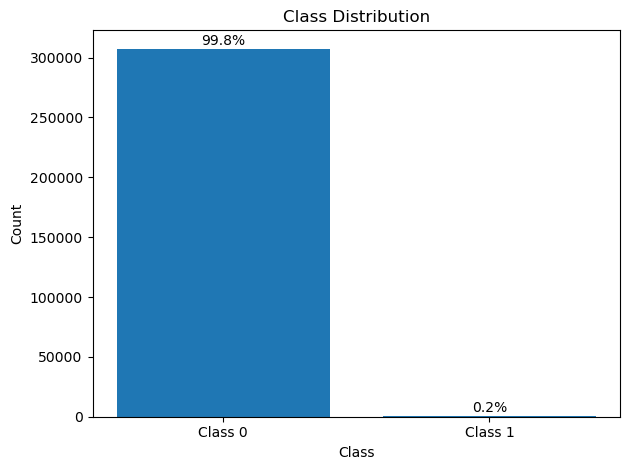
\includegraphics[width=0.8\linewidth]{figures/Imbalaced data for aflag.png}
    \caption{Class Distribution for $\bar{\alpha}$ on 31st January. In the overall 308,178 data, class 0 accounts for 99.8\% of the samples, while Class 1 represents only 0.2\%, indicating a severe class imbalance.}
    \label{fig: aflag_class_distribution}
\end{figure}

SMOTE (Synthetic Minority Over-sampling Technique) is an advanced oversampling method that generates synthetic samples of the minority class by interpolating between existing ones. However, since SMOTE connects both inliers and outliers arbitrarily, it may lead to a sub-optimal decision boundary, especially in high-dimensional and noisy datasets of our case. To better fit our dataset, I adopt a SMOTE variant called KMeansSMOTE, which applies KMeans clustering before performing oversampling. This clustering step groups similar samples together and generates synthetic data based on cluster density. For our high-frequency and extremely imbalanced data, KMeansSMOTE helps prevent synthetic samples from being generated in sparse or noisy regions, and creates more informative minority class samples that reflect the local data structure.
Let $\mathcal{X}_{\text{min}} = \{x_1, \dots, x_{N_{\text{min}}}\} \subset \mathbb{R}^d$ be the minority class. KMeansSMOTE proceeds as follows:

Apply KMeans to $\mathcal{X}_{\text{min}}$ with $k$ clusters:
  \[
  \min_{\{C_j\}} \sum_{j=1}^k \sum_{x \in C_j} \|x - \mu_j\|^2, \quad \mu_j = \frac{1}{|C_j|} \sum_{x \in C_j} x
  \]

For each cluster $C_j$, compute:
  \[
  \text{Density}_j = \frac{|C_j|}{\text{avg\_intra\_dist}(C_j)}, \quad w_j = \frac{1/\text{Density}_j}{\sum_{i} 1/\text{Density}_i}
  \]
where avg\_intra\_dist is the average pairwise distance within $C_j$. Set $n_j = \lfloor w_j \cdot n_{\text{gen}} \rfloor$.

For each $C_j$, repeat $n_j$ times:
  \[
  \tilde{x} = x + \lambda (x^{\text{NN}} - x), \quad \lambda \sim \mathcal{U}(0, 1)
  \]
where $x, x^{\text{NN}} \in C_j$ are randomly selected minority points and one of its $k$ nearest neighbors.

Building upon the foundation laid in the balanced class, weighted loss functions are implemented during the machine learning training process to focus on the accuracy of class 1. For example, in XGBoost, the weight is applied to the loss function by assigning a higher importance to the misclassification of class 1 samples. Specifically, the objective function includes a weighted logistic loss where the weight $w_i$ for each instance increases if the sample belongs to the target class, influencing both the gradient and Hessian in the boosting process. Additionally, take GRU-based RNN for another example, class weights are introduced in the binary cross-entropy loss function. The loss becomes:
\[
\mathcal{L} = -w_1 \cdot y \cdot \log(\hat{y}) - w_0 \cdot (1 - y) \cdot \log(1 - \hat{y})
\]
where $w_1$ and $w_0$ are the weights for class 1 and class 0, respectively, $y$ is the true label, and $\hat{y}$ is the predicted probability. This weighted loss penalizes the model more for errors on class 1, guiding it to pay more attention to the target class during training.

Anomaly filter methods are also applied to highlight the regions around aggressive trading events. This thesis presents a window-based filter function to extract time segments centered around class 1 instances. Specifically, for each sample with a non-missing DIRECTION label, which means there is at least one trade recorded, a window of certain milliseconds is defined. All entries within this time range are included for training. This method ensures that the model is exposed to a richer context around potential anomalies and enhances the learning of class 1 patterns in the high-frequency setting. In our practical implementation, I integrate an anomaly detection function alongside KMeansSMOTE across different models. This ensures that imbalanced class problem are handled without conflict in each model and maintains balanced class distributions consistently between the models.

\begin{algorithm}[H]
\caption{Window-Based Anomaly Filter} \label{al: window-based}
\begin{algorithmic}[1]
\State \textbf{Input:} Data with timestamps and labels; window size $\delta$
\State \textbf{Output:} Filtered data around class 1 instances
\For{each timestamp $t$ where \texttt{DIRECTION} is not NaN}
    \State Define window: $[t - \delta/2,\ t + \delta/2]$
    \State Find all rows within this window and add their indices to \texttt{result\_indices}
\EndFor
\State \Return rows corresponding to \texttt{result\_indices}
\end{algorithmic}
\end{algorithm}


\section{Prediction Model: An XGBoost-Enhanced Neural Hawkes Process Framework}
This thesis proposes an XGBoost-enhanced Neural Hawkes Process framework combining class imbalance solutions, neural encoder, and stochastic modeling to predict aggressive trades under extreme class imbalance. The framework is designed to first resolve class imbalance through resampling in XGBoost, then integrate nonlinear and long-range feature dependencies, which are extracted from recurrent neural networks, into the calculation of intensity in Hawkes processes. 

To depict the general workflow of our framework, Figure~\ref{fig:data-flow-diagram} presents the overall workflow of our framework, combining both the training (estimation) phase and the testing phase. More detailed and clearly separated diagrams will be discussed in Section~\ref{sec:data-flow}. The framework begins with an XGBoost classifier trained to identify aggressive trade events from limit order book features displayed in Table~\ref{tb: overall dataset for training}. 

To address the extreme class imbalance in the dataset, KMeansSMOTE is applied during training to generate synthetic minority samples in a structure-aware manner, ensuring a more balanced and representative training set. The first-filtered output of the XGBoost model, alongside features, is then fed into a Gated Recurrent Unit (GRU), which acts as a historical market state encoder. The GRU transforms the inputs into a compact hidden state that captures nonlinear dependencies and long-range dynamics in condition of temporal logic ($T$) and market features ($S$, $M$, $V_A^{1}$, $V_A^{1}$, $\bar{\delta}_S$, $\bar{\delta}_M$, $\sigma_S$, $\sigma_M$, $r_V$). This hidden state is used to condition the intensity function $\lambda(t)$ of a neural Hawkes process. Unlike classical Hawkes models based on additive exponential kernels, the intensity here is dynamically modulated by the GRU output, allowing the model to flexibly capture evolving market microstructure behavior. As a result, the process becomes a conditional point process, where the estimation of parameters is informed by both structured and balanced output of the XGBoost model and the latent dynamics embedded in recent order book activity.

In the first stage, I employ XGBoost to predict $\bar{\alpha}$ on the full trading day using limit order book features in Table~\ref{tb: overall dataset for training}. To address the extreme class imbalance and get potential aggressive trade rows, I apply KMeansSMOTE before training. This first classifier aims to identify as many true trade points as possible (high recall) and increase the proportion of minor class in the output. The model filters out most of the non-aggressive instances (class 0) and provides a broad set of aggressive trade activity candidates. This output serves two purposes: it reduces the candidate space for aggressive trade prediction, and its feature importance guides the selection of input features for subsequent models.

In the second stage, I train a GRU-based recurrent neural network to get the hidden state formula of the two market scenarios as mentioned in Table~\ref{tb: aflag_meaning} (aggressive and non-aggressive). The GRU model is trained on a balanced dataset constructed using a window-based anomaly filter function around class 1 labels as presented in Algorithm~\ref{al: window-based}. This stage further refines the prediction of aggressive trades by deep learning networks. The GRU hidden state captures these invisible market conditions that traditional Hawkes can not see, but that critically affect event intensity.

In the final stage, I apply a neural Hawkes process to analyze a more dynamic estimation and prediction of aggressive trades. The Hawkes model captures the temporal clustering of aggressive trade events and demonstrates interpretable output in the form of aggressive and non-aggressive trade intensity and probability. This significantly compensates for the limited ability of machine learning models. I also incorporate a condition based on MN trade execution information: if an internal order is filled within certain milliseconds window, it increases the likelihood of a nearby aggressive trade. This step not only enhances the final accuracy and F1 score, but also produces a more interpretable, precise and inclusive prediction set.

Overall, this framework effectively predicts rare aggressive trades by combining class imbalance solution, market states features, temporal dependency, and clustering modeling. It predicts the intensity and final pattern of aggressive and non-aggressive events. The following parts of the section elaborate each of the three components and discuss the combined contribution of the predictive framework.

\begin{figure}[H]
    \centering
    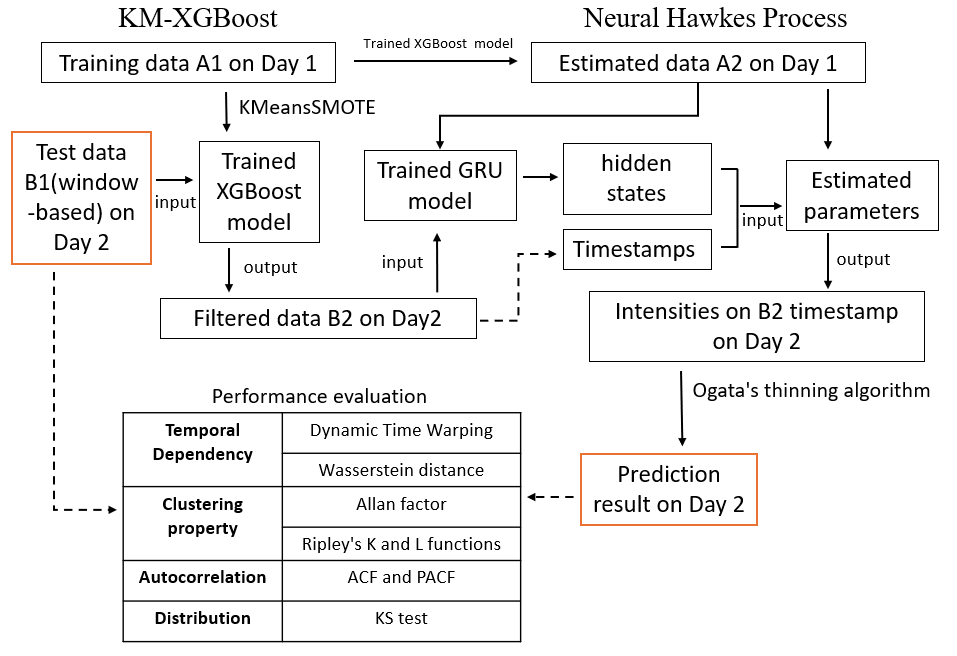
\includegraphics[width=0.8\textwidth]{figures/data_flow1.png}
    \caption{Data flow of the full pipeline from raw data to final prediction, combining both training and testing stages.}
    \label{fig:data-flow-diagram}
\end{figure}


\subsection{XGBoost with KMeansSMOTE Filtering (KM-XGBoost)}
XGBoost is a tree-based ensemble learning method that builds a sequence of decision trees to minimize a specified loss function. With a gradient boosting logic, each new tree is trained on the residual errors of the current model, effectively correcting its mistakes by following the negative gradient of the loss. 

XGBoost is a strong overall model, which includes features that make it especially practical and powerful in real-world applications. \cite{XGBoost_2016} compare XGBoost with some other popular classifiers, and find XGBoost helps prevent overfitting through built-in regularization, can handle sparse data automatically without preprocessing, and is optimized for speed and memory efficiency, making it well-suited for large-scale datasets with imbalanced data. XGBoost can capture nonlinear patterns that logistic regression cannot, and handles sparse data with native sparsity-aware algorithms. Compared to GBM (Traditional Gradient Boosting Machines), XGBoost significantly outperforms them in training time (up to 10x faster) and often in test accuracy. In the context of Kaggle competitions, XGBoost outperforms neural networks, especially in tabular data, and top entries use XGBoost rather than deep learning models \citep{XGBoost_2016}. It represents that XGBoost is easier to tune and more robust to hyperparameter choices in those settings and less data-hungry than deep neural nets.

The underlying objective function of XGBoost can be explained as follows: a loss term and a regularization term. It is defined as:

\begin{equation}
\mathcal{L}(\phi) = \sum_{i=1}^{n} l(y_i, \hat{y}_i^{(t)}) + \sum_{k=1}^{t} \Omega(f_k)
\end{equation}

Where $l$ is a differentiable convex loss function, such as the logistic loss for binary classification. It measures the difference between the true label $y_i$ and the predicted value $\hat{y}_i^{(t)}$ at iteration $t$. The second term, $\Omega(f_k)$, is a regularization function that penalizes the complexity of each added tree $f_k$.

The regularization term is defined as:

\begin{equation}
\Omega(f) = \gamma T + \frac{1}{2} \lambda \|w\|^2
\end{equation}

Here, $T$ denotes the number of leaves in the regression tree, $w$ represents the vector of scores assigned to the leaves, and $\gamma$, $\lambda$ are regularization parameters that control the penalty on the number of leaves and the magnitude of leaf weights respectively. If $T$ is larger, it gives better data fitting and gets penalties by $\lambda$ and $\lambda \|w\|^2$, avoiding overfitting.

This thesis uses GridSearchCV and cross-validation to find the best hyperparameters for the XGBoost model. GridSearchCV is a module from the Python library scikit-learn \citep{scikit-learn2011}, which performs an ergodic search over a grid of hyperparameter values. It combines this with cross-validation, a technique that splits the training data into multiple folds. In each round, one fold is used for validation and the others for training. This helps to evaluate the model performance more fairly and avoids overfitting to one specific subset of data. 

Algorithm~\ref{alg: grid_search} demonstrates the setup of hyperparameter tuning. The search is conducted over three values each for $n\_estimators$ (number of boosting rounds), $max\_depth$, $learning\_rate$, and $min\_child\_weight$. One fixed value of $scale\_pos\_weight$, which was computed based on the class imbalance ratio. The evaluation metric used is ROC-AUC, which is especially suitable for imbalanced classification tasks. A 3-fold cross-validation ($cv=3$) is applied, and the search is performed in parallel using all available CPU cores ($n\_jobs=-1$) for efficiency. To give more focus on aggressive trades, instance weights are manually adjusted before fitting: class 1 (aggressive trades) is assigned a higher weight (100.0), while class 0 (non-aggressive trades) receives a weight of 1. This weighting helps the model pay more attention to aggressive trades during training.

% \begin{algorithm}[H]
% \caption{Grid Search with Cross-Validation for XGBoost} \label{alg: grid_search}
% \begin{algorithmic}[1]
%     \State Define base XGBoost model with fixed settings:
%     \Statex \hspace{\algorithmicindent} \texttt{use\_label\_encoder=False}, \texttt{eval\_metric='logloss'}, \texttt{random\_state=42}
%     \State Define hyperparameter grid:
%     \Statex \hspace{\algorithmicindent} \texttt{n\_estimators} $\in \{100, 300, 500\}$
%     \Statex \hspace{\algorithmicindent} \texttt{max\_depth} $\in \{3, 5, 7\}$
%     \Statex \hspace{\algorithmicindent} \texttt{learning\_rate} $\in \{0.01, 0.02, 0.05\}$
%     \Statex \hspace{\algorithmicindent} \texttt{min\_child\_weight} $\in \{3, 5, 7\}$
%     \Statex \hspace{\algorithmicindent} \texttt{scale\_pos\_weight} = computed class imbalance ratio
%     \State Initialize GridSearchCV with:
%     \Statex \hspace{\algorithmicindent} scoring metric: ROC-AUC
%     \Statex \hspace{\algorithmicindent} cross-validation folds: 3
%     \Statex \hspace{\algorithmicindent} parallel jobs: all CPUs (\texttt{n\_jobs=-1})
%     \State Compute sample weights:
%     \Statex \hspace{\algorithmicindent} weight = 100.0 for aggressive trades
%     \Statex \hspace{\algorithmicindent} weight = 1.0 for non-aggressive trades
%     \State Fit model to resampled training data using \texttt{sample\_weight}
%     \State Return best hyperparameters and cross-validated model
% \end{algorithmic}
% \end{algorithm}

\begin{algorithm}[H]
\caption{Grid Search with Cross-Validation for XGBoost}\label{alg: grid_search}
\begin{algorithmic}[1]
    \State Define base XGBoost model:
    \Statex \hspace{\algorithmicindent} \texttt{use\_label\_encoder=False}, \texttt{eval\_metric='logloss'}, \texttt{random\_state=42}
    \State Define base XGBoost model with fixed settings:
    \Statex \hspace{\algorithmicindent} \texttt{use\_label\_encoder=False}, \texttt{eval\_metric='logloss'}, \texttt{random\_state=42}
    \State Define hyperparameter grid:
    \Statex \hspace{\algorithmicindent} \texttt{n\_estimators} $\in \{100, 300, 500\}$
    \Statex \hspace{\algorithmicindent} \texttt{max\_depth} $\in \{3, 5, 7\}$
    \Statex \hspace{\algorithmicindent} \texttt{learning\_rate} $\in \{0.01, 0.02, 0.05\}$
    \Statex \hspace{\algorithmicindent} \texttt{min\_child\_weight} $\in \{3, 5, 7\}$
    \Statex \hspace{\algorithmicindent} \texttt{scale\_pos\_weight} = computed class imbalance ratio
    \State Initialize GridSearchCV with:
    \Statex \hspace{\algorithmicindent} scoring metric: ROC-AUC
    \Statex \hspace{\algorithmicindent} parallel jobs: all CPUs (\texttt{n\_jobs=-1})
    \State Compute sample weights:
    \Statex \hspace{\algorithmicindent} weight = 100.0 for aggressive trades
    \Statex \hspace{\algorithmicindent} weight = 1.0 for non-aggressive trades
    \ForAll {hyperparameter combinations in grid}
        \For{fold $k = 1$ to $K$ (e.g. 3)}
            \State Split data into training set $D_{\text{train}}^{(k)}$ and validation set $D_{\text{val}}^{(k)}$
            \State Train model on $D_{\text{train}}^{(k)}$ using sample weights
            \State Evaluate ROC-AUC on $D_{\text{val}}^{(k)}$
        \EndFor
        \State Compute average ROC-AUC across $K$ folds
    \EndFor
    \State Select the hyperparameter set with the highest average ROC-AUC
    \State Re-train final model on full training set using selected hyperparameters
\end{algorithmic}
\end{algorithm}

The architecture of XGBoost encourages the model to fit the data effectively with awareness of class focus, while avoiding overfitting by controlling model complexity. This results in a faster and more practical training process.

In our study, KMeansSMOTE is applied to the training data to address class imbalance before feeding it into XGBoost. XGBoost is then used to predict $\bar{\alpha}$ and to generate feature importance scores. These scores serve as a reference for selecting relevant features in the subsequent neural network training. This feature selection step helps reduce model complexity and focuses the learning process on the most informative patterns. The input-output workflow of this process can be summarized as follows:
\begin{itemize}
  \item \textbf{Input:}  
  The model receives a resampled dataset obtained by applying KMeansSMOTE to the original data presented in Table~\ref{tb: overall dataset for training}. The resampling adjusts the class distribution to approximately 3:7 (aggressive:non-aggressive). Input features include engineered features $S$, $M$, $V_A^{1}$, $V_A^{1}$, $\bar{\delta}_S$, $\bar{\delta}_M$, $\sigma_S$, $\sigma_M$, $r_V$.

  \item \textbf{Model Configuration:}  
  An XGBoost classifier is trained using hyperparameters selected via GridSearchCV. The final model configuration is:
  \begin{itemize}
    \item \texttt{n\_estimators} = 500
    \item \texttt{max\_depth} = 7
    \item \texttt{min\_child\_weight} = 5
    \item \texttt{learning\_rate} = 0.05
    \item \texttt{scale\_pos\_weight} = computed imbalance ratio
    \item \texttt{eval\_metric} = 'logloss'
    %\item \texttt{random\_state} = 42
  \end{itemize}

  \item \textbf{Output:}  
  The model outputs a binary prediction for each record in the time window of a given trading day, indicating whether the event is likely to be an aggressive trade (\texttt{class = 1}). The output gives a more balanced class dataset, with the class 1 (aggressive trade) accounting for approximately 10\% of the whole data.

\end{itemize}



%-------------------------GRU-----------------------------
\subsection{Gated Recurrent Units (GRU)-based RNN}
% what's GRU
To model the nonlinear and long-range sequential dynamics in condition of market features of aggressive trades, I employ a recurrent neural network (RNN) based on GRU. GRU is a type of neural network designed to work with sequential data alongside engineered features, such as time series, sentences, or trading records. Unlike standard models that treat each input independently, a GRU learns from past information and current input at the same time. When I deal with data that unfolds over time, like a series of trades, it's important to understand how earlier events influence later ones. For example, an aggressive trade might be more likely to happen now if the spread was very low several ticks ago. 

% why GRU not others
GRU is a simplified variant of the Long Short-Term Memory (LSTM) network, designed to capture long-range dependencies while using fewer parameters and computational resources \citep{GRU2014}. It has a simplified architecture with two gates: the update gate and reset gate. The update gate controls how much of the previous hidden state should be retained, and the reset gate determines how much of the past information to forget. The two gates allow the model to remember or forget past information as needed, crucial for understanding market patterns in order book data. Since it lacks the forget gate, compared to LSTM, GRU has fewer parameters and faster training times, making it more efficient for larger datasets. In many cases, the performance difference between LSTM and GRU is not significant, and GRU is often preferred due to its simplicity and efficiency. 

In our study, I adopt a GRU architecture instead of the LSTM structure used by \cite{lalor_event-based_2025} because our problem involves fewer event types, but much higher frequent dynamics, where fast and robust convergence is critical. More specifically, Table~\ref{tab:gru_vs_lstm} compares the use of GRU with the LSTM approach used by \cite{lalor_event-based_2025}.

\begin{table}[H]
\centering
\caption{Comparison of LSTM-Based Model vs. GRU-Based Model}
\begin{tabular}{p{3cm} p{5.5cm} p{5.5cm}}
\toprule
\textbf{Aspect} & \textbf{LSTM-Based Model} & \textbf{GRU-Based Model} \\
\midrule
\textbf{Data Domain} & Stock LOBSTER data (lower tick frequency, long time span) & FX spot market data (millisecond frequency, short time window) \\
\textbf{Purpose} & Simulates all 12 LOB event types & Predicts binary outcome \\
\textbf{Complexity} & High: expressive but computationally intensive & Low: efficient and sufficient for task-specific modeling \\
\textbf{Training Time} & Slower convergence; more resource intensive & Faster training; lightweight structure \\
\textbf{Overfitting Risk} & High: due to model size and variable performance across assets & Lower: binary setting with consistent performance \\
\bottomrule
\end{tabular}
\label{tab:gru_vs_lstm}
\end{table}

On the one hand, the LSTM-based approach is designed to handle a large and diverse set of 12 LOB event types. This level of event complexity and inter-type interaction needs a more complicated but also heavier architecture like LSTM. In contrast, our setting focuses on a simpler and more specific prediction task. Our training dataset contains just two types of market scenarios (aggressive vs. non-aggressive trades). I do not simulate all LOB events but instead focus on binary classification. Therefore, the computational burden of LSTM is unnecessary, and the more efficient GRU offers a faster and equally expressive alternative for our goal.

On the other hand, \cite{lalor_event-based_2025} relied on stock data from LOBSTER. It is relatively lower tick frequencies compared to higher-frequent FX spot markets. As a result, fast and robust convergence is critical. GRU is a more suitable RNN to predict aggressive trade pattern in the high frequency FX spot market.


% why hidden states matter and math formulas
GRU helps the model remember those earlier patterns by giving a hidden state. It is a memory storage that is updated at each step in the sequence. The core assumption behind using an RNN is that the current output depends not only on the current input but also on the historical sequence of past inputs. Formally, a GRU updates its hidden state through gating mechanisms that regulate the flow of information, allowing it to selectively retain or forget past information as needed. It can consist of multiple stacked GRU layers and be followed by a dense output layer. Each GRU layer returns sequences to preserve the full temporal structure across time steps. The model is trained to minimize a weighted mean squared error (MSE) loss. 
\begin{equation}
    \mathcal{L} = \frac{1}{N} \sum_{i=1}^{N} \sum_{t=\text{warmup\_steps}}^{T} w_{i,t} \left( y_{i,t} - \hat{y}_{i,t} \right)^2
    \label{eq:GRU loss function}
\end{equation}
    where
\begin{equation}
    w_{i,t} =
    \begin{cases}
    w_\text{nozero}, & \text{if } y_{i,t} \neq 0 \\
    w_\text{zero}, & \text{if } y_{i,t} = 0
    \end{cases}
    \label{eq:weight in GRU loss}
\end{equation}
    
In Equation.~\ref{eq:GRU loss function} and \ref{eq:weight in GRU loss}, higher importance is given to nonzero targets to emphasize the prediction of aggressive behaviors. Furthermore, the initial warmup steps are ignored in each sequence when calculating the loss. During this phase, hidden state representations are still developing, and their predictions are often noisy \citep{lambrechts2023warmingrecurrentneuralnetworks}. This can prevent the model from being penalized during its early and uncertain predictions.

The GRU works through four simple steps. First, the reset gate $r_t$ decides how much of the previous memory to forget when creating new information. If values close to 0, it forgets most of the past and values, while values closing to 1 mean remember everything. Next, the update gate $z_t$ acts as a mixing controller that determines how much to blend old memory with new information. The candidate hidden state $\tilde{h}_t$ represents the proposed new memory based on the current input. Finally, the most important part, actual hidden state $h_t$, is computed as a weighted average between the old memory and the new candidate. It controls how much of the old memory should be used to create new information, and how much should the memory be updated with this new information.
\begin{align}
    % Reset Gate
    r_t = \sigma(W_r \cdot [h_{t-1}, x_t] + b_r) \\
    % Update Gate
    z_t = \sigma(W_z \cdot [h_{t-1}, x_t] + b_z) \\
    % Candidate Hidden State
    \tilde{h}_t = \tanh(W_h \cdot [r_t \odot h_{t-1}, x_t] + b_h) \\
    % Final Hidden State
    h_t = (1 - z_t) \odot h_{t-1} + z_t \odot \tilde{h}_t
\end{align}

% input and output
In our study, the model is trained to capture hidden states which can keep useful memory of past inputs. These hidden states are later used as dynamic inputs for the Hawkes process. It works well enough for our binary trade prediction task and helps connect market features with intensity estimation. The input-output workflow of this process can be summarized as follows:

\begin{itemize}
  \item \textbf{Input:}  
  An anomaly filter is applied to the raw dataset. For each record with a valid \texttt{DIRECTION} label, a fixed-width time window is constructed. All entries falling within this window are collected to form a training sample. This ensures the filtered dataset maintains approximately 10\% aggressive trades, aligning with the XGBoost classifier's output distribution.

  Before training, features and labels are scaled using \texttt{MinMaxScaler()}, and sequences are reshaped with a fixed length of 3000 time steps. The training is conducted using a batch size of 32.

  \item \textbf{Model Configuration:}  
  A GRU-based model is defined using Keras \texttt{Sequential()}:
  \begin{itemize}
    \item First layer: GRU with 1024 units, returning sequences.
    \item Second layer: Fully connected \texttt{Dense} layer with sigmoid activation.
    \item Optimizer: RMSprop with learning rate $10^{-3}$
    \item Loss function: custom \texttt{loss\_mse\_warmup} to exclude initial warmup steps from the loss.
  \end{itemize}

  The model is trained with \texttt{model.fit()} using a generator that yields sequences, over 6 epochs with 6 steps per epoch. These settings are selected based on convergence behavior.

  \item \textbf{Output:}  
  After training, a hidden state extraction function is applied to retrieve the dynamic GRU hidden states at each timestamp for both aggressive (class 1) and non-aggressive (class 0) trades. These hidden states are then used to condition the intensity function in the subsequent Hawkes process.
\end{itemize}




\subsection{Neural Hawkes Process}
% what is Hawkes and how our neural HP nice
The Hawkes process is a self-exciting point process that models events happening over time. It is called 'self-exciting' because each event can make future events more likely (or less likely) to happen soon after. This is different from normal classification models that give a yes-or-no answer. The Hawkes process gives a time-varying intensity function, written as $\lambda(t)$, which represents the conditional probability density of the occurrence of an event in the immediate future \citep{bacry_hawkes_2015}. 

I use a neural Hawkes process to improve this traditional model. Instead of using fixed formulas, I let a neural network reinforce the calculation of the intensity function. This makes the model more flexible and able to fit complex patterns, like how the memory of past trades changes over time and how the historical market features affect current situations. By the way of GRU learning hidden patterns in the order book sequence, using its hidden states inside the Hawkes model allows us to connect trading signals with time-based predictions in a natural way. This design is especially useful for modeling latent, event-driven and clustering data like trades in the FX market.


% why integrate hidden states instead of traditional HP
The neural Hawkes model extends traditional Hawkes process which uses a fixed parametric form for the intensity function. Traditional Hawkes processes use simple exponential kernels model the event intensity function. However, in real markets, especially in high-frequency trading, these patterns can be much more complex and change over time. By using hidden states from a GRU-based RNN, I let the model learn a flexible and feature-driven representation of market dynamics, which is new and novel. The GRU encodes recent history, including both the timing and features of past events, into a hidden state. This hidden state is then used to compute the event intensity $\lambda(t)$ in the Hawkes model. In this way, the influence of past events is no longer predefined, but instead learned directly from the data. Integrating GRU hidden states with the Hawkes process turns the model into a neural version, called a neural Hawkes process. In our case, this gives the model the ability to adapt to irregular and complex trade patterns, while still keeping the time-based prediction structure of Hawkes models. This makes it more suitable for FX markets, where trade behavior can change quickly and does not always follow simple rules but latent status.


% how hidden states and trade aware are used in math formula
A key innovation in our approach is the hidden state integration and trade-aware intensity adjustment. In the following part of this section, I explain the mathematical interpretation of intensity function in our neural Hawkes process. I first use the GRU hidden state $h_t$ to adjust the intensity. This allows the model to include latent market conditions that traditional Hawkes process cannot detect, but which may critically strongly influence the intensity of a new event. Moreover, I add another term to the intensity function: if one of our own trades occurs within a short time window near time $t$, I increase the intensity $\lambda(t)$ by a small boost $\delta$. This reflects the idea that our own trading activity may increase the chance of other events happening soon after. The adjusted conditional intensity function is given by:

\begin{equation}
    \lambda_k(t) = (\mu_k + \sum_{j=1}^{K} \sum_{t'_j=T}^{t-1} \alpha_{kj} e^{-\beta_{kj}(t - t'_j)}) \times \log(1+e^{h_k(t)}) + \delta \cdot \mathbf{1}_{\{\exists \tau \in \mathcal{T}_{\text{own}},\ |t - \tau| \leq \Delta \}}
    \label{eq:intensity}
\end{equation}

\begin{equation}
    \log \mathcal{L} = \sum_{i=1}^{N} \log \lambda_{t_i}^{k_i} - \sum_{k=1}^{K} \int_{0}^{T} \lambda_t^{k} \, dt
    \label{eq:log_likelihood_hawkes}
\end{equation}

In Equation~\ref{eq:intensity}, $\lambda_k(t)$ is the intensity of event $k$ at time $t$. The term $\mu_k$ is the baseline intensity, which stays constant for that event type across all time. The parameters $\alpha_{kj}$ and $\beta_{kj}$ control the influence of past events: $\alpha_{kj}$ measures how much an event of type $j$ excites the occurrence of type $k$, and $\beta_{kj}$ is the decay rate that reduces this influence over time. $K$ is the total set of events. The sum over $t'_j$ from fixed time $T$ up to time $t-1$ means I are considering a certain length of the past events history before time t. I assume that only one event can happen at each timestamp, so there is no overlap. The first part $(\mu_k + \sum_{j=1}^{K} \sum_{t'_j=T}^{t-1} \alpha_{kj} e^{-\beta_{kj}(t - t'_j)})$ is the same structure as the traditional Hawkes process. It gives the intensity based on a decaying memory of past events. 

However, I extend this with two additional terms. The first is a neural modulation term \( \log(1 + e^{h_k(t)}) \), where \( h_k(t) \) is the hidden state from the GRU. This component allows the intensity to be adjusted based on recent market signals learned from sequential patterns. The second is a spike term $\delta$. If one of our own trades occurred within a small time window \( \Delta \) around time \( t \), I increase the intensity by a fixed boost \( \delta \). This term reflects the idea that our own trading activity may influence the short-term behavior of the market.

In Equation~\ref{eq:log_likelihood_hawkes}, \( \log \mathcal{L} \) is the log-likelihood function of our model. The first term sums the log intensity values at all observed event times \( t_i \), for their corresponding event types \( k_i \). $N$ is the total number of observed events in the time interval \([0, T]\). $t_i$ is the timestamp of the $i$-th observed event. These are the times at which events occur, such that $0<t_1<t_2<...<t_i<...<T$.
The second term subtracts the integral of the intensity function over the full time period \([0, T]\) for all event types. The combination of the two terms ensures that the model explains observed events well without overestimating event frequency in general. It is worth to note that the integral $\int_{0}^{T} \lambda_t^{k} \, dt$ is part of the exact log-likelihood in this continuous-time setting. It measures the total 'expected number of events' over time and penalizes models that expect too many events between actual ones.


% how I use it
During the implementation, I model each trade event using a one-hot encoded vector to distinguish between aggressive and non-aggressive trades. Specifically, I define the event types as:
\begin{center}
\begin{tabular}{lll}
(1, 0) & : & Non-aggressive trade \\
(0, 1) & : & Aggressive trade \\
\end{tabular}
\end{center}
This encoding provides a clear way to display the type of trading behavior at each timestamp. Passive trades are grouped with no-trade events because the interest is only in predicting aggressive trades.

I define the number of event types with the variable \texttt{n\_dims=2}, and initialize the key parameters of the neural Hawkes process as follows:

\begin{itemize}
    \item \( \mu_k = 0.1 \): the baseline intensity for each type.
    \item \( \alpha_{kj} = 0.2 \): the excitation parameter measuring how much a type-\( j \) event influences the likelihood of a future type-\( k \) event.
    \item \( \beta_{kj} = 1.0 \): the decay rate that controls how fast the influence of past events fades over time.
\end{itemize}

I choose to include the 50 most recent events before each time step to strike a balance between capturing sufficient historical influence and maintaining computational efficiency. This window size is also consistent with the memory length encoded by the GRU hidden states used in our neural intensity modulation. For training, I minimize the negative log-likelihood defined in Equation~\ref{eq:log_likelihood_hawkes}. I use the L-BFGS-B optimization method, which is well suited for problems with parameter bounds. This procedure also respects positivity and numerical stability constraints of the intensity function because in Equation~\ref{eq:intensity} $\mu$ and $\alpha$ are all positive, and no other terms contribute any negative value.

% Ogata's thinning algorithm
Once the intensity function \( \lambda(t) \) is fitted, I decide aggressive trade patterns using \textbf{Ogata's thinning algorithm}. This method allows us to sample event times from a continuous-time multivariate point process by checking whether each proposed event fits the modeled intensity. At each candidate time \( t \), I follow these steps:

\begin{enumerate}
    \item I compute the GRU hidden state \( h(t) \) and use it, along with past events, to calculate the conditional intensity vector \( \boldsymbol{\lambda}(t) \in \mathbb{R}^K \), where \( K \) is the number of event types.
    
    \item I define an upper-bound intensity \( \lambda_{\text{max}} \) for thinning. If no events have occurred yet, I set \( \lambda_{\text{max}} = \sum_{k=1}^{K} \mu_k \). Otherwise, I use \( \lambda_{\text{max}} = \sum_{k=1}^{K} \lambda_k(t) \), based on current computed intensities.

    \item A candidate time \( t \) is accepted if a random number \( u \sim \text{Uniform}(0,1) \) satisfies:
    \[
    u < \frac{\sum_{k=1}^{K} \lambda_k(t)}{\lambda_{\text{max}}}
    \]
    
    \item If accepted, the event type is sampled from a categorical distribution proportional to the individual intensities:
    \[
    p_k = \frac{\lambda_k(t)}{\sum_{j=1}^{K} \lambda_j(t)}
    \]
    where \( p_k \) is the probability of sampling event type \( k \) at time \( t \).

    \item The resulting event \( (t, \text{type}, h(t)) \) is recorded for future simulation steps.
\end{enumerate}
This ensures that the resulting sample reflects the target intensity function \( \lambda(t) \). As noted by \citet{magris_simulation_nodate}, Ogata's modified thinning algorithm remains one of the most efficient and widely adopted techniques for simulating self-exciting point processes.



% why it's more interpreable
It is important to note that this modeling approach gives interpretable results, which is essential for real-world applications like MN's FX backtesting system. Unlike black-box models, where it is difficult to explain why a prediction is made, the Hawkes process provides an explicit intensity function that describes the probability of aggressive trades over time. A higher intensity in the aggressive trade dimension directly corresponds to a higher likelihood of predicting such a trade. This makes it easier to explain the model's behavior to traders or portfolio managers. Instead of saying 'the machine decided', I can point to specific factors like recent market activity, hidden states learned from GRU, or our own past executions that contributed to the increased intensity. The model not only captures temporal clustering, but also integrates latent market conditions and the effect of our own executions.


% \section{Whole Framework}
\section{Overall Data Flow} \label{sec:data-flow}
First, I provide a more detailed explanation of Figure~\ref{fig:data-flow-diagram}, which shows the complete data flow of the framework. It includes KMeansSMOTE XGBoost and the Neural Hawkes Process. On the left side, training data A1 from Day 1 is used to train the KM-XGBoost classifier. KMeansSMOTE is applied to improve class imbalance. Normally the final training dataset contains  over 400,000 rows and 13 columns. The trained model is then used to filter aggressive trades on window-based (like 30 minutes or 1 hour) test data B1 from Day 2, producing the output data B2.

On neural Hawkes process side, estimated data A2 is functioned by an anomaly detection for class balance. Then it is processed by a GRU model to extract hidden states. After that, estimation of the parameters is implemented. The filtered data B2 from the XGBoost stage is used to compute the event intensities on B2 timestamps. These intensities are passed through Ogata's thinning algorithm to promote the final aggressive trade predictions.

The final prediction result is evaluated against the true events using various metrics, including dynamic time warping, Wasserstein distance, Allan factor, Ripley's K and L functions, autocorrelation (ACF/PACF), and KS test. These metrics cover different dimensions such as temporal dependency, clustering, and distribution.

Specially, 

\begin{figure}[H]
\centering
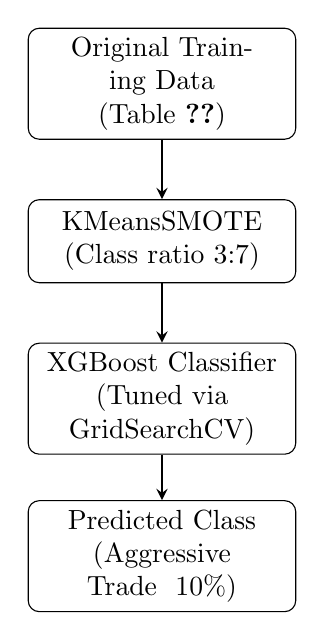
\begin{tikzpicture}[node distance=2cm]

\node (data) [block] {Original Training Data \\ (Table~\ref{tb: overall dataset for training})};
\node (resample) [block, below of=data] {KMeansSMOTE \\ (Class ratio 3:7)};
\node (xgboost) [block, below of=resample] {XGBoost Classifier \\ (Tuned via GridSearchCV)};
\node (output) [block, below of=xgboost] {Predicted Class \\ (Aggressive Trade ~10\%)};

\draw [arrow] (data) -- (resample);
\draw [arrow] (resample) -- (xgboost);
\draw [arrow] (xgboost) -- (output);

\end{tikzpicture}
\caption{XGBoost input-output workflow for aggressive trade prediction.}
\label{fig:xgboost-flow}
\end{figure}

\begin{figure}[H]
\centering
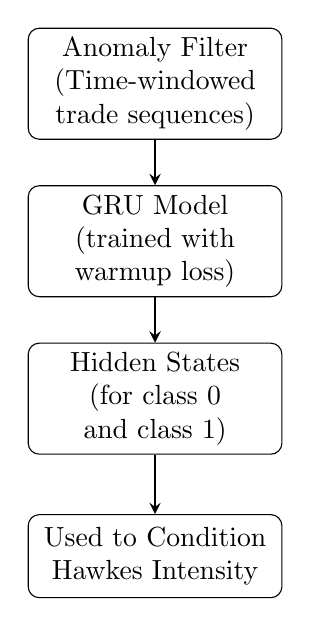
\begin{tikzpicture}[node distance=2cm]

    \tikzstyle{block} = [rectangle, draw, text width=8.5em, align=center, rounded corners, minimum height=3em]
    \tikzstyle{arrow} = [thick,->,>=stealth]

    \node (filtered) [block] {Anomaly Filter\\ (Time-windowed trade sequences)};
 
    \node (gru) [block, below of=filtered] {GRU Model\\ (trained with warmup loss)};

    \node (hidden) [block, below of=gru] {Hidden States\\ (for class 0 and class 1)};

    \node (hawkes) [block, below of=hidden] {Used to Condition\\ Hawkes Intensity};

    \draw [arrow] (filtered) -- (gru);
    \draw [arrow] (gru) -- (hidden);
    \draw [arrow] (hidden) -- (hawkes);

\end{tikzpicture}
\caption{Input-output flow of the GRU-based encoder.}
\label{fig:gru-flow}
\end{figure}

The input-output workflow of this process can be summarized as follows:
\begin{figure}[H]
\centering
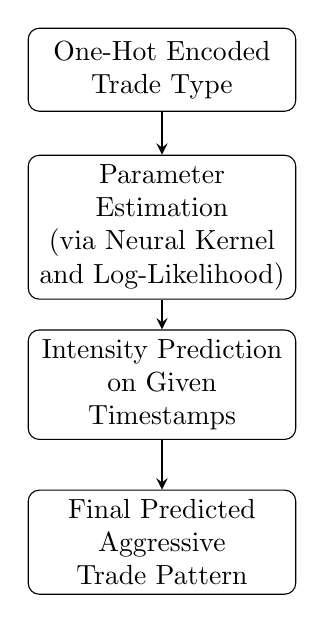
\begin{tikzpicture}[node distance=2cm]
    \tikzstyle{block} = [rectangle, draw, text width=9em, align=center, rounded corners, minimum height=3em]
    \tikzstyle{arrow} = [thick,->,>=stealth]
    \node (onehot) [block] {One-Hot Encoded\\ Trade Type};
    \node (estimate) [block, below of=onehot] {Parameter Estimation\\ (via Neural Kernel and Log-Likelihood)};
    \node (predict) [block, below of=estimate] {Intensity Prediction\\ on Given Timestamps};
    \node (output) [block, below of=predict] {Final Predicted\\ Aggressive Trade Pattern};

    \draw [arrow] (onehot) -- (estimate);
    \draw [arrow] (estimate) -- (predict);
    \draw [arrow] (predict) -- (output);

\end{tikzpicture}
\caption{Input-output flow of the Neural Hawkes Process.}
\label{fig:neural-hawkes-flow}
\end{figure}

\section{Evaluation Metrics} \label{sec:evaluation-metrics}
This section introduces the metrics useful to evaluate how well the predicted aggressive trades resemble the actual ones in the market. Traditional classification metrics, such as precision and recall, assume that each predicted event must match one true event exactly. However, in our case, MN accepts that the prediction of an aggressive trade does not have to be exactly on the timestamp in the data, but can be in an interval around this moment. Thus, I care more about the temporal patterns and distributional behavior of events. For this reason, I include other metrics that can measure similarity in terms of clustering, alignment, and statistical distribution.

As shown in Table~\ref{tb:Evaluation Metrics}, I organize the evaluation into five categories: classification-based metrics, temporal dependency metrics, clustering metrics, autocorrelation, distributional statistical tests.

\begin{table}[h]
\centering
\begin{tabular}{|l|l|l|}
\hline
\textbf{Category} & \textbf{Metric} & \textbf{Purpose} \\
\hline
Classification & Confusion Matrix & Pointwise event match \\
Classification & Precision, Recall, F1-score & Basic prediction quality \\
Temporal Dependency & DTW & Flexible pattern alignment \\
Temporal Dependency & Wasserstein Distance & Distributional shift in timing \\
Temporal Dependency & Fréchet Distance & Curve shape similarity \\
Clustering & Allan Factor & Burstiness and overdispersion \\
Clustering & Event Counts & Count variation in time bins \\
Clustering & Ripley's K Function & Multi-scale clustering test \\
Autocorrelation & Autocorrelation Analysis & Memory and repeated patterns \\
Distributional Test & KS Test & Statistical distribution equality \\
Distributional Test & KL Divergence & Information loss in distributions \\
\hline
\end{tabular}
\caption{Summary of Evaluation Metrics}\label{tb:Evaluation Metrics}
\end{table}

\subsection{Classification-based Metrics}
The confusion matrix shows the number of correctly and incorrectly predicted events. It includes true positives (TP), false positives (FP), true negatives (TN), and false negatives (FN). TP are cases where the model correctly predicts an aggressive event, meaning both the actual and predicted values are one. FP occur when the model predicts an aggressive event, but no actual event happens. TN are when the model correctly predicts non-aggressive trades, with both actual and predicted values being zero. FN happen when an actual aggressive event occurs, but the model fails to detect it, resulting in a missed event. These values help measure how many real events were captured and how many predictions were wrong.

Based on the confusion matrix, I calculate precision, recall, and F1-score. Precision is the proportion of correct predictions out of all predicted events. Recall is the proportion of actual events that were correctly predicted. F1-score is the harmonic mean of precision and recall. However, in our case, these values are not very meaningful because aggressive events are rare and exact matches are unlikely. Still, I include them for completeness.

\subsection{Temporal Dependency Metrics}
Temporal dependency metrics evaluate how well the predicted aggressive trade sequence follows the timing and rhythm of the actual sequence. These metrics are useful when the goal is to match general behavior.

Dynamic Time Warping (DTW) is a technique that allows flexible alignment between two sequences by warping the time axis, making it suitable for comparing patterns that may not align perfectly in time \citep{muller2007dtw}. Wasserstein Distance, also known as Earth Mover's Distance, measures how much 'effort' is needed to move one event timing distribution into another. It is useful for comparing the overall position and spread of events. Fréchet Distance measures the similarity between two event trajectories, considering the order and path taken by events. It focuses more on the global shape than local alignment.

Together, these three metrics provide a more complete evaluation of temporal similarity. DTW captures local flexibility and pattern alignment, Wasserstein Distance reflects distributional shift in timing, and Fréchet Distance focuses on overall shape.

\subsection{Clustering Metrics}
Clustering metrics test whether events happen close together in time, which is a common behavior in financial markets, especially for trader behaviors.

The Allan Factor measures how much the event counts vary in fixed time windows. Values close to one suggest random behavior, while higher values indicate clustering. Event Counts per Fixed Window analyze how many events happen in each time bin (e.g., 1 second, 5 seconds). Ripley's K Function is used to check clustering at multiple time scales. If the K value is higher than expected under randomness, then clustering is present.

Each of these metrics captures clustering from a different perspective. The Allan Factor focuses on overdispersion in event counts over time, Event Counts per Fixed Window provide direct insight into local density, and Ripley's K Function examines clustering across multiple time scales. Using all three allows us to evaluate both short-term and long-term clustering behavior, making the analysis more reliable than using any single metric alone.

\subsection{Autocorrelation Metrics}
Autocorrelation metrics check whether events are dependent on previous events. In market microstructure, it is common to see memory or self-excitation in order flows. Autocorrelation Analysis measures the correlation between an event and its past values. If the correlation is significant at short lags, it suggests that events are not independent.

\subsection{Distributional Statistical Tests}
These tests compare the statistical properties of predicted and actual events. The Kolmogorov-Smirnov (KS) Test compares the cumulative distributions of inter-arrival times. A high p-value means there is no significant difference between the two. Kullback-Leibler Divergence (KL) measures how much information is lost when one distribution is used to represent another. Lower values mean the two distributions are more similar.

While the KS Test provides a formal statistical test for distributional similarity, KL Divergence offers a continuous measure of how much the distributions differ in shape and information. By combining both, I can assess distributional similarity, which leads to a more balanced evaluation than relying on either one alone.


